\documentclass[border=0.8ex,svgnames,tikz]{standalone}
\usepackage{amsmath,mathtools}
\usepackage{fontspec}
\setmainfont{Source Serif 4}
\setsansfont{Source Sans 3}
\setmonofont{Source Code Pro}

\usetikzlibrary{fit,positioning,calc,shapes.misc}

\begin{document}
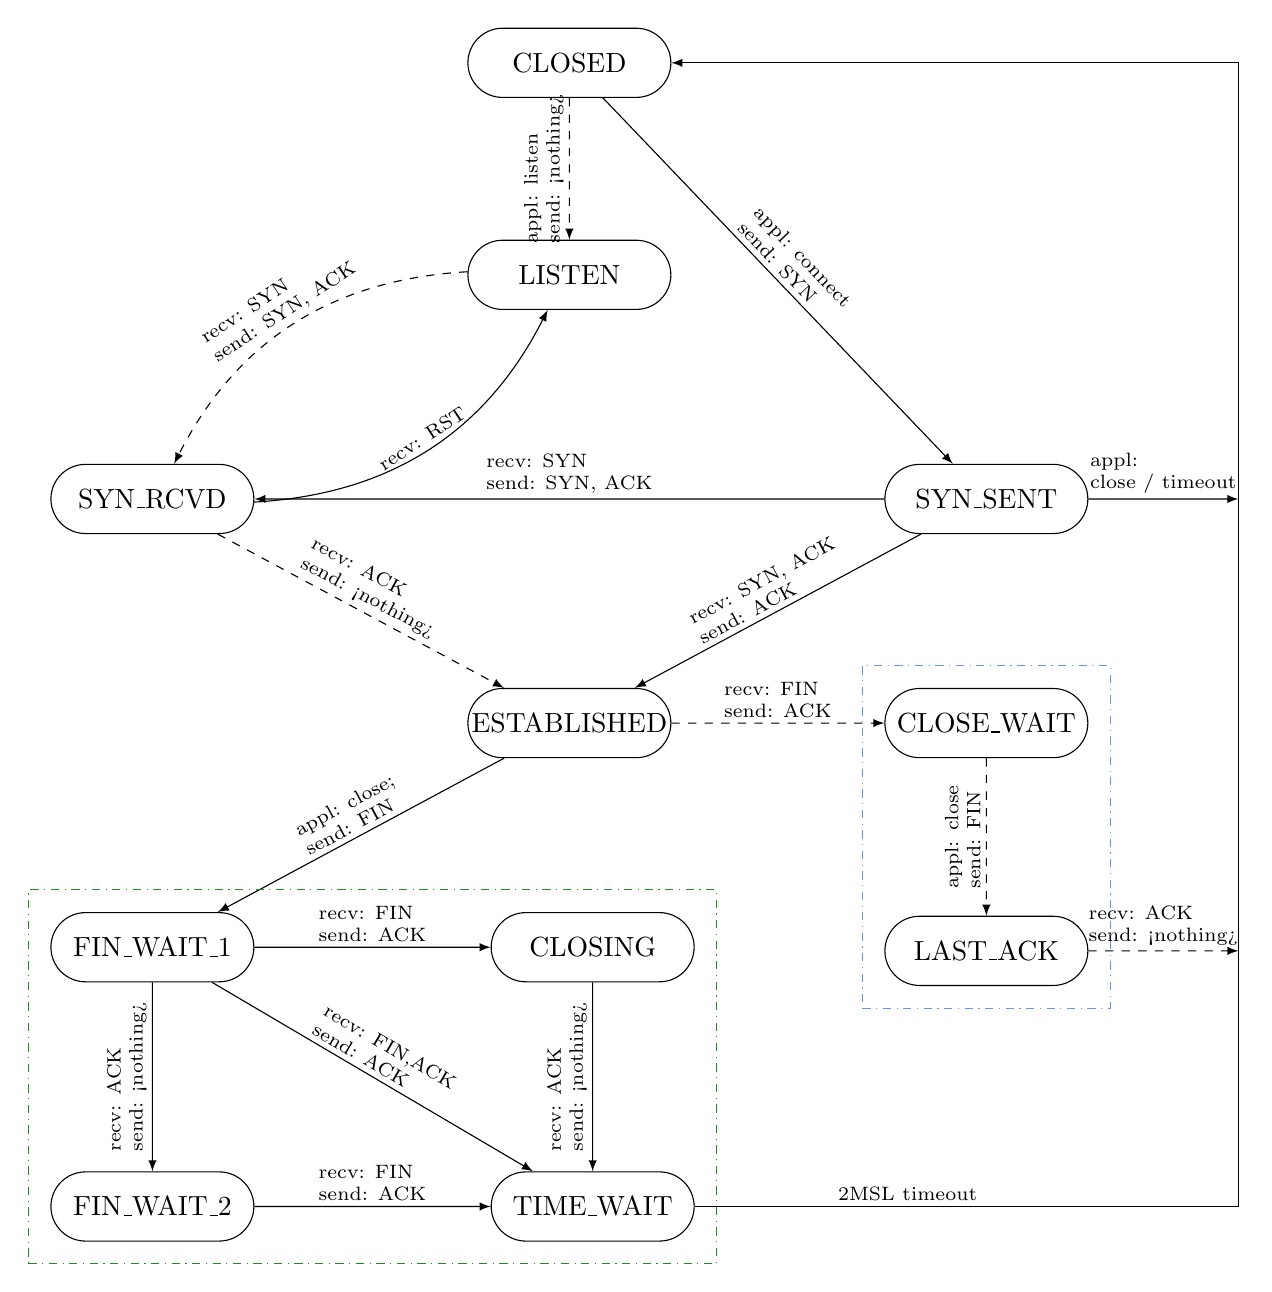
\begin{tikzpicture}
  \begin{scope}[
    every node/.style={
      draw,
      minimum width=8em,
      minimum height=2.5em,
      rounded rectangle,
      rounded rectangle arc length=180,
      font=\normalsize,
    },
    ]
    \node (syn-rcvd) {SYN\_RCVD};
    \node[right=8.0 of syn-rcvd] (syn-sent) {SYN\_SENT};
    \node[above=2.4 of $(syn-rcvd)!0.5!(syn-sent)$] (listen) {LISTEN};
    \node[below=2.4 of $(syn-rcvd)!0.5!(syn-sent)$] (established) {ESTABLISHED};
    \node[above=1.8 of listen] (closed) {CLOSED};
    \node[below=2.4 of syn-sent,anchor=center] (close-wait) {CLOSE\_WAIT};
    \node[below=2.0 of close-wait] (last-ack) {LAST\_ACK};
    \node[below=4.8 of syn-rcvd] (fin-wait-1) {FIN\_WAIT\_1};
    \node[right=3.0 of fin-wait-1] (closing) {CLOSING};
    \node[below=2.4 of fin-wait-1] (fin-wait-2) {FIN\_WAIT\_2};
    \node[right=3.0 of fin-wait-2] (time-wait) {TIME\_WAIT};
  \end{scope}
  \coordinate (passive-end) at ($(last-ack)+(3.2,0)$);
  \coordinate (active-end) at ($(syn-sent)+(3.2,0)$);
  \begin{scope}[
    every path/.style={draw,dashed,>=latex},
    every node/.style={
      above,
      sloped,
      draw=none,
      fill=none,
      inner sep=0.45ex,
      align=left,
      font=\scriptsize,
    },
    ]
    \path[->]
    (closed) edge node{appl: listen\\send: <nothing>} (listen)
    (listen) edge[bend right] node{recv: SYN\\send: SYN, ACK} (syn-rcvd)
    (syn-rcvd) edge node{recv: ACK\\send: <nothing>} (established)
    (established) edge node{recv: FIN\\send: ACK} (close-wait)
    (close-wait) edge node{appl: close\\send: FIN} (last-ack)
    (last-ack) edge node{recv: ACK\\send: <nothing>} (passive-end);
  \end{scope}
  \begin{scope}[
    every path/.style={draw,>=latex},
    every node/.style={
      above,
      sloped,
      draw=none,
      fill=none,
      inner sep=0.45ex,
      align=left,
      font=\scriptsize,
    },
    ]
    \path[->]
    (closed) edge node{appl: connect\\send: SYN} (syn-sent)
    (syn-sent) edge node{recv: SYN\\send: SYN, ACK} (syn-rcvd)
    (syn-sent) edge node{recv: SYN, ACK\\send: ACK} (established)
    (syn-sent) edge node{appl:\\close / timeout} (active-end)
    (syn-rcvd) edge[bend right] node{recv: RST} (listen)
    (established) edge node{appl: close;\\send: FIN} (fin-wait-1)
    (fin-wait-1) edge node{recv: FIN\\send: ACK} (closing)
    (fin-wait-1) edge node{recv: FIN,ACK\\send: ACK} (time-wait)
    (fin-wait-1) edge node{recv: ACK\\send: <nothing>} (fin-wait-2)
    (closing) edge node{recv: ACK\\send: <nothing>} (time-wait)
    (fin-wait-2) edge node{recv: FIN\\send: ACK} (time-wait);
    \path[->] (time-wait) -| (passive-end) -- (active-end) |- (closed);
    \path (time-wait) ++(4,0) node{2MSL timeout};
  \end{scope}
  \begin{scope}[fit node/.style n args={2}{
      fit=#1,
      inner sep=0.8em,
      rectangle,
      dash dot,
      draw=#2,
    }]
    \node[fit node={(close-wait)(last-ack)}{CornflowerBlue}]{};
    \node[fit node={(fin-wait-1)(time-wait)}{ForestGreen}]{};
  \end{scope}
\end{tikzpicture}
\end{document}
